
%%%%%%%%%%%%%%%%%%%%%%%%%%%%%%%%%%%%%%%%%%%%%%%%%%%%%%%%%%%%%%%%%%%%%%%%%%%%%%%%
%2345678901234567890123456789012345678901234567890123456789012345678901234567890
%        1         2         3         4         5         6         7         8

\documentclass[letterpaper,10pt,conference]{ieeeconf}  % Comment this line out if you need a4paper

%\documentclass[a4paper, 10pt, conference]{ieeeconf}      % Use this line for a4 paper

\IEEEoverridecommandlockouts                              % This command is only needed if 
                                                          % you want to use the \thanks command

\overrideIEEEmargins                                      % Needed to meet printer requirements.

% See the \addtolength command later in the file to balance the column lengths
% on the last page of the document

% The following packages can be found on http:\\www.ctan.org
\usepackage{graphics} % for pdf, bitmapped graphics files
%\usepackage{epsfig} % for postscript graphics files
%\usepackage{mathptmx} % assumes new font selection scheme installed
%\usepackage{times} % assumes new font selection scheme installed
\usepackage{amsmath} % assumes amsmath package installed
\usepackage{amssymb}  % assumes amsmath package installed

%\usepackage{graphicx}
%\usepackage{amsmath}
%\usepackage{amssymb}
%\usepackage{amsthm}
\usepackage{mathtools}
\usepackage{array}
\usepackage{dsfont}
%\theoremstyle{definition}
%\newtheorem{example}{Example}
\usepackage{subfigure}
\usepackage{multirow}
\usepackage[subnum]{cases}
\usepackage{overpic}
\usepackage{color}
\usepackage{upgreek}
\usepackage{textcomp}
\usepackage{cite}
\usepackage{bm}

\frenchspacing

\title{\LARGE \bf
Algorithm for finding optimal gait patterns for a gecko-inspired soft robot
%Algorithm for predicting the pose of a gecko-inspired soft robot for a given reference input
}

\author{Lars Schiller and Arthur Seibel% <-this % stops a space
%\thanks{The authors are with Workgroup on System Technologies and Engineering Design Methodology, Hamburg University of Technology, 21073 Hamburg, Germany
\thanks{Authors are with Workgroup on System Technologies and Engineering Design Methodology, Hamburg University of Technology, 21073 Hamburg, Germany
			 {\tt\small arthur.seibel@tuhh.de}
			 %{\tt\small \{arthur.seibel,lars.schiller\}@tuhh.de}
				}%
}

\begin{document}

\maketitle
\thispagestyle{empty}
\pagestyle{empty}

%%%%%%%%%%%%%%%%%%%%%%%%%%%%%%%%%%%%%%%%%%%%%%%%%%%%%%%%%%%%%%%%%%%%%%%%%%%%%%%%

\begin{abstract}
%Dieses Paper stellt einen Algorithmus vor, der die Pose eines aus weichen Biegeaktuatoren bestehenden Roboters zu einem gegebenen Referenzinput vorhersagen kann.
%Dieser Algorithmus wird dann dazu verwendet, optimale Laufmuster für den geraden Gang und für eine Kurve zu entdecken.
%So konnte das Laufmuster für den geraden Gang um den Faktor 1.5 verbessert werden und ein neues Laufmuster für die Rotation auf der Stelle entdeckt werden.

This paper presents an algorithm that can predict the pose of a robot consisting of soft bending actuators to a given reference input.
This algorithm is then used to find optimal gait patterns for the straight gait and for a curve.
The existing gait pattern for the straight gait could be improved by a factor of 1.5 and a new gait pattern for the rotation on the spot could be discovered.

\end{abstract}

%%%%%%%%%%%%%%%%%%%%%%%%%%%%%%%%%%%%%%%%%%%%%%%%%%%%%%%%%%%%%%%%%%%%%%%%%%%%%%%%


\newcommand{\mbeq}{\overset{!}{=}}

\makeatletter
\renewcommand*\env@matrix[1][*\c@MaxMatrixCols c]{%
  \hskip -\arraycolsep
  \let\@ifnextchar\new@ifnextchar
  \array{#1}}
\makeatother




\section{Introduction}

Due to the fact that the behaviour of soft materials is difficult to predict with conventional methods, an algorithm based on a geometric optimization problem is presented.
The algorithm can be used to predict the actual pose of a soft robot for a given reference input.
Figure~\ref{fig:example} is taken as an example. The initial position is shown in black. 
The individual limbs of the robot have a certain bending angle and all feet are fixed.
Now the torso of the robot should be actuated. 
If only the bending angle of the torso is changed, the grey dashed pose is obtained. 
Obviously, the two rear feet are no longer in the same position. 
Since these feet are fixed, the robot will behave differently in reality. 
In fact, it's much more likely to take up the grey pose. 
Although the bending angles of all limbs have changed, the condition that all feet remain motionless has been fulfilled.

\begin{figure}[h]
\centering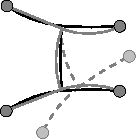
\includegraphics[scale=1]{../Pics/intro/intro.pdf}
\caption{Example Usage}
\label{fig:example}
\end{figure}



\section{Predicting the pose for a given reference input}
In order to let the robot take a pose
%, i.\,e., a position and orientation, 
the user has nine degrees of freedom at his disposal: 
the correspondending pressures for the five bending angles $\alpha_i$ of the limbs $i=1,\dots,5$ and the state of the fixation actuators $f_j \in \{0,1\}$ of the feet $j=1,\dots,4$.
For the unloaded state, a calibration function can be formulated for each limb, which maps the input pressure on the bending angle (under load, this function no longer needs to be valid).
But the input pressure can be seen as an reference for the bending angle.
Accordingly, a reference input $\bm{r}$ can be described by

\begin{equation}
\bm{\alpha}_{\textnormal{ref}} = \left[~ \alpha_{\textnormal{ref},1}~\alpha_{\textnormal{ref},2}~\alpha_{\textnormal{ref},3}~\alpha_{\textnormal{ref},4}~\alpha_{\textnormal{ref},5}~\right]^\top
\end{equation}

\begin{equation}
\bm{f} = \left[~f_1~f_2~f_3~f_4~\right]^\top
\end{equation}


\begin{equation}
\bm{r} = \left[~\bm{\alpha_{\textnormal{ref}}}^\top~\bm{f}^\top~\right].
\end{equation}

%
%\begin{equation}
%\alpha_{\textnormal{clb},i} = \textnormal{map}_i(p_i)
%\end{equation}

However, this information is not sufficient to describe the robot's actual pose.
%The exact position and orientation of at least one foot must be known.
Experiments have shown that the bending angle of a limb can vary significantly  at the same pressure level due to the softness of the used material. 
The length of a limb can also differ.
In order to describe the pose of the robot, the actual bending angles $\bm{\alpha}$: 
\begin{equation}
\bm{\alpha} = \left[ \alpha_1~\alpha_2~\alpha_3~\alpha_4~\alpha_5 \right]^\top,
\end{equation}
the actual lengths of the individual limbs $\bm{\ell$}: 
\begin{equation}
\bm{\ell} = \left[ \ell_1~\ell_2~\ell_3~\ell_4~\ell_5 \right]^\top,
\end{equation}
and the orientation of the robot's center point $\varepsilon$ must be known (see Fig.~\ref{fig:model}).
These quantities are defined as the variable to be optimized:
\begin{equation}
\bm{x} = \left[~\bm{\alpha}^\top~\bm{\ell}^\top~\varepsilon~\right]^\top.
\end{equation}

Furthermore, the position of (at least) one fixed foot ($f_j \mbeq 1$) must be known.
Then, the pose of the robot $\bm{\rho}$ can be determined under the assumption of a constant curvature by drawing arcs with the corresponding lengths and angles.
A pose can therefore be described in generally as a function of $\bm{x}$ and the position 
$\bm{P}=[\bm{p}_1~\bm{p}_2~\bm{p}_3~\bm{p}_4]^\top = [\bm{p}_x~\bm{p}_y]^\top \in \mathbb{R}^{4 \times 2}$ and state $\bm{f}$ of all feet:
\begin{equation}
\bm{\rho} = \left[\bm{x}~\bm{P}~\bm{f} \right].
\end{equation}



For a given feasible initial pose, the next pose must be determined so that all fixed feet do not move.
This can be achieved within a certain margin by deviating the bending angle from the reference angle and deviating the actual length from the nominal length.
To describe this mathematically, a new index $k$ is introduced, which assigns the quantities to a specific time step.
The new positions of the fixed feet $\bm{P}_{k}$ are assumed to be the positions from the previous pose $\bm{P}_{k-1}$.
This can be used to define the constraint for the next pose.
All newly fixed feet must have the same position as in the previous step:
\begin{equation}
\big|\big|\textnormal{diag}(\bm{f}_k)(\bm{P}_{k} - \bm{P}_{k-1})\big|\big|_2 \mbeq 0,
\label{eq:constraint}
\end{equation}


%\begin{equation}
%\bm{p}_k \left(\bm{x},~\bm{p}_{k-1},~\bm{f}_k \right).
%\end{equation}

%Please note that if this condition is met, at least one foot per time step always remains motionless.
%Thus, at least one foot position of the new pose is determined from the beginning and thus dependent on the previous pose.
%As a result, all poses of a gait are dependent on the initial position.
%\begin{equation}
%\bm{\rho}_t = \textnormal{fun}\left(\bm{x}_t,~\bm{r}_{j,0} \right).
%\end{equation}

It has already been mentioned that the bending angles $\bm{\alpha}$ and the lengths of the limbs $\bm{\ell}$ are quite variable. 
By defining 
\begin{equation}
\bm{\ell}_n = \left[ \ell_{n,1}~\ell_{n,2}~\ell_{n,3}~\ell_{n,4}~\ell_{n,5} \right]^\top
\end{equation}
as the vector containing the nominal length of each limb, it is possible to quantify the length deviation.
The orientation angles of the fixation actuators $\bm{\varphi}$ also have a certain margin.
The value of the orientation angles can be calculated as a function of $\bm{\alpha}$ and $\varepsilon$ (well, basically as a function of $\bm{x}$):
\begin{equation}
\bm{\varphi}(\bm{\alpha}, \varepsilon) = \eqref{eq:phi_calc},
\end{equation}
where the exact formula is given in the appendix~\eqref{eq:phi_calc}.
Now a objective function $\sigma$ can be formulated which quantifies the deviations of length, angle and orientation:
%\begin{equation}
%obj(\bm{x}) = w_{len}\sqrt{\sum_i \left( \ell_{n,i} - \ell_i \right)^2} 
%+ w_{ang} \sqrt{\sum_i \left( \varphi_i - \alpha_i \right)^2}
%+ w_{ori} \sqrt{\sum_i \textnormal{if}~f_i:~\left( c_{i,j-1} - c_{i, j} \right)^2}
%\label{eq:objective_function}
%\end{equation}

\begin{equation}
\begin{array}{ccl}
\sigma(\bm{x}_{k}) &=& 
w_\ell\big| \bm{\ell}_{k} - \bm{\ell}_n \big|_2
+ w_\alpha\big| \bm{\alpha}_{k} - \bm{\alpha}_{\textnormal{ref},k} \big|_2 \\
&&+ w_\varphi \big| \textnormal{diag}(\bm{f}_k) ( \bm{\varphi}_{k} - \bm{\varphi}_{k-1}) \big|_2
\end{array}.
\label{eq:objective_function}
\end{equation}
The weighting factors can be interpreted physically.
To do so, the weighting factor $w_\ell$ describes the elasticity of the limbs and $w_\alpha$ the bending stiffness of the limbs.
The term weighted by $w_\varphi$ describes the difference between the orientation of the newly fixed feet compared to the orientation in the previous time step.
This can be seen as a dimension for the torsional stiffness of the fixation actuators.
The objective function can be seen as a measure of the robot's inner stress.
Therefore it is called $\sigma$ referring to the nomenclature in mechanical engineering.
The new pose can now be determined by solving the non-linear optimization problem:

\begin{equation}
\begin{split}
&\min_{\bm{x}_k \in \mathcal{X}} ~ \sigma(\bm{x}_k) \\
&subjected~to~~~
\big|\big|\textnormal{diag}(\bm{f}_k)(\bm{P}_{k} - \bm{P}_{k-1})\big|\big|_2 = 0.
\end{split}
\end{equation}
Here  $\mathcal{X}$ describes the set of allowed values.
Each quantity inside $\bm{x}$ has bounds, which are given in the following table:

\begin{center}
\begin{tabular}{c|c}
var & bounds \\
\hline
$\bm{\alpha}$ & $\left[ \bm{\alpha_{\textnormal{ref}}}-b_\alpha,~\bm{\alpha_{\textnormal{ref}}}+b_\alpha \right]$ \\
$\bm{\ell}$ & $\left[ (1-b_\ell)\bm{\ell}_n,~(1+b_\ell)\bm{\ell}_n \right]$ \\
$\varepsilon$ & $\left[ 0^\circ,~ 360^\circ \right]$ \\
\end{tabular}
\end{center}
These bounds can be tuned with the scalars $b_\alpha$ and $b_\ell$.
For solving the problem, for example the \texttt{SLSQP}-Algorithm provided by the python package \texttt{scipy.optimize} can be used.
Note that the evaluation of the objective function~\eqref{eq:objective_function} is quite cheap. 
The expensive part is the evaluation of the constraint function~\eqref{eq:constraint}, since the calculation of all feet positions for a given $\bm{x}$ is opulent and outlined in the appendix~\eqref{eq:F1_start}--\eqref{eq:F1_end}.

In summary, it is possible to set up a function that can predict the next pose of the robot, depending on the reference input and the previous pose:
\begin{equation}
\bm{\rho}_k = [\bm{x}_k~\bm{P}_k~\bm{f}_k] = \textnormal{fun}_{\mathcal{P}}\left( \bm{r}_k, \bm{\rho}_{k-1} \right)
\end{equation}
This function can be tuned by the parameter set $\mathcal{P}$ given in the following table:
\begin{center}
\begin{tabular}{l|p{7cm}}
$\mathcal{P}$ & description \\
\hline
$b_\alpha$ & allowed absolute deviation of the bending angle to the reference angle \\
$b_\ell$ & allowed percentage deviation of the length to the nominal length \\
$w_\ell$ & costs of the length deviation / Youngs-Modulus of the material \\
$w_\alpha$ & costs of the bending angle deviation / bending stiffness of the limbs\\
$w_\varphi$ & costs of the orientation angle deviation / torsional stiffness of the fixation actuators\\
\end{tabular}
\end{center}



\begin{figure}
\centering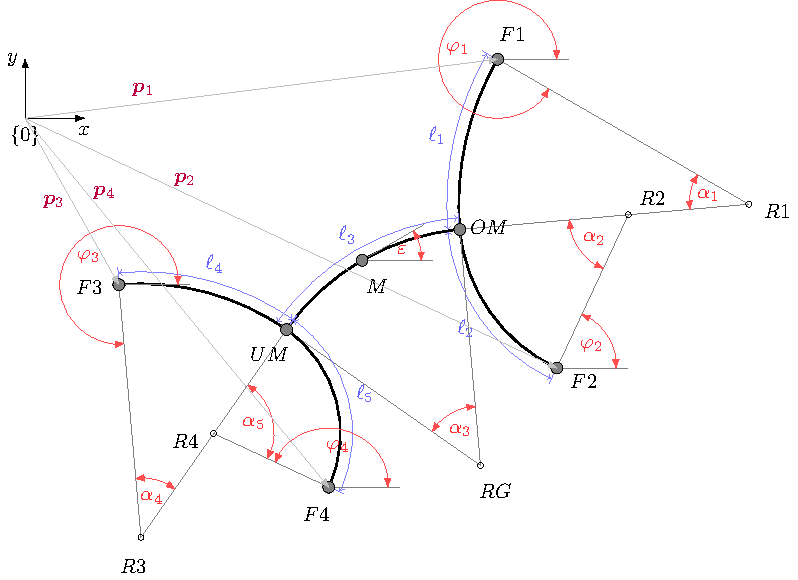
\includegraphics[scale=1]{../Pics/model/model.pdf}
\caption{Nomencalture}
\label{fig:model}
\end{figure}


\section{Finding optimal gait patterns}

%Der vorgesttele Algorithmus kann nun dazu verwendet werden neue Laufmuster zu finden.
%Da er die Möglichkeit bietet vorherzusagen, welche Pose der Roboter bei gegebenem Referenz Input einnehmen wird, ist er durch rekursive Anwendung in der Lage alle zugehörigen Posen des Roboters zu einer Sequenz von Referenz Inputs zu prädiktieren.
%

The presented algorithm can now be used to find new gait patterns.
Since it provides the ability to predict the robot's pose for a given reference input, it is also able to predict all associated poses to a sequence of reference inputs by recursive application.

%Allerdings wird eine gültige Initialpose benötigt, um den vorgestellten Algorithmus rekursiv anwenden zu können.
%Gültig in dem Sinne, dass die Längen und Biegewinkel der Glieder innerhalb des gültigen Bereichs liegen.
%Die Bedingung~\eqref{eq:constraint}, dass die im vorhergegangenen Schritt fixierten Füße nicht bewegt werden dürfen, ist an dieser Stelle hinfällig, da kein vorhergegangener Schritt existiert.
%Zur Berechnung einer gültigen Initialpose können initiale Biegewinkel $\bm{\alpha}_0$, initiale Gliederlängen $\bm{\ell}_0$ und Orientierung $\varepsilon_0$ frei gewählt werden.
%Dabei empfiehlt es sich für die Gliederlängen $\bm{\ell}_0 = \bm{\ell}_n$ zu wählen, da so die "innere Spannung" der Initialpose $\sigma(\bm{x}_0) = 0$ ist.
%Die Fußpositionen $\bm{P}_0$ ergeben sich dann durch Anwendung der Gleichungen~\eqref{eq:F1_start}--\eqref{eq:F1_end}.
%Dabei muss die initiale Koordinate des vorderen linken Fußes $\bm{p}_{1,0}$ vorgegeben werden.

However, a valid initial pose is required to apply the presented algorithm recursively.
Valid in the sense that the lengths and bending angles of the limbs are within the valid range.
The condition~\eqref{eq:constraint}, that the feet fixed in the previous step may not be moved, is void at this point, since no previous step exists.
To calculate a valid initial pose, initial bending angles $\bm{\alpha}_0$, initial limb lengths $\bm{\ell}_0$ and orientation $\varepsilon_0$ can be freely defined.
For the limb lengths $\bm{\ell}_0 = \bm{\ell}_n$ is recommended, as the " inner stress " of the initial pose is $\sigma(\bm{x}_0) = 0$.
The feet positions $\bm{P}_0$ result then by application of equations~\eqref{eq:F1_start}--\eqref{eq:F1_end}.
Thereby the initial coordinate of the front left foot $\bm{p}_{1,0}$ must be provided.


\begin{equation}
\begin{array}{ccl}
\bm{\rho}_0 &=& 
\left[
\begin{array}{c|c|c}
\bm{x}_0 & \bm{P}_0 & \bm{f}_0
\end{array}
\right] \\
&=&
\left[
\begin{array}{c|c|c}
\bm{\alpha}_0 ~ \bm{\ell}_n ~ \varepsilon_0  & 
\bm{P}(\bm{\alpha}_0, \bm{\ell}_n, \varepsilon_0, \bm{p}_{1,0}) & 
1~0~0~0
\end{array}
\right]
\end{array}
\end{equation}

%Ein Laufmuster besteht aus einer ebensolchen Sequenz aus Posen, die in Dauerschleife eingenommen werden.
%Um nun eine optimale Abfolge von Referenz Inputs zu finden, muss erst einmal definiert werden, was optimal ist.
%Dies kommt ganz darauf an, welche Art von Laufmuster gesucht wird. 
%im Folgenden werden zwei Beispiele vorgestellt.


A gait pattern consists of a sequence of poses taken in a loop with a certain number of cycles.
To find an optimal sequence of reference inputs, it is first necessary to define what is optimal.
This depends entirely on the type of gait pattern we are looking for. 
Two examples are presented below.


\subsection{Straight Gait}
%Es ist sinnvoll anzunehmen, dass ein symmetrisches Laufmuster am ehesten zu einem geradlinigen Gang führen wird.
%Symmetrisch in dem Sinne, dass auf eine bestimmte Pose stets die zur Längsache gespiegelte Pose folgt.
%Außerdem sind die Fixierungszustände der Füße ebenfalls von vornherein bekannt, da für einen symmetrischen Gang stets die diagonal gegenüberliegenden Füße fixiert sein müssen (siehe vorhergegangene Forschungsarbeiten - \cite{PA_Schiller}).
%Damit besitzt das Laufmuster nur fünf Unbekannte, nämlich die Referenzwinkel der ersten Pose -- alle weiteren Posen innerhalb des Laufmusters sind Spiegelbilder.




It is reasonable to assume that a symmetrical gait pattern will most likely lead to a straigth gait.
Symmetrical in the sense that a certain pose is always followed by a pose mirrored to the longitudinal axis.
In addition, the state of fixation of the feet is also known from the outset, since the diagonally opposite feet must always be fixed for a symmetrical gait (see previous research work - \cite{PA_Schiller}).
Thus, the running pattern has only five unknowns, namely the reference angles of the first pose -- all other poses within the gait pattern are mirror images.
Therefore the variable to be optimized can be defined as:
\begin{equation}
\bm{y} = 
\begin{bmatrix}
\alpha_{\textnormal{ref},1}& \alpha_{\textnormal{ref},2}&\alpha_{\textnormal{ref},3}&\alpha_{\textnormal{ref},4}&\alpha_{\textnormal{ref},5}
\end{bmatrix} .
\end{equation}

%Mit diesen Annahmen kann eine Struktur für das noch unbekannte Laufmuster für den geradlinigen Gang mit $n$ Zyklen $\bm{R}_\mathcal{S}^n \in \mathbb{R}^{2n \times 9} $ vorgegeben werden:

With these assumptions a structure for the still unknown straight gait pattern with $n$ cycles $\bm{R}_\mathcal{S}^n \in \mathbb{R}^{2n \times 9} $ can be given as:
\begin{equation}
\bm{R}_\mathcal{S}^n(\bm{y})
%=
%\left[
%\begin{array}{c}
%\bm{r}_1 \\
%\bm{r}_2 \\
%\hline
%\bm{r}_3 \\
%\bm{r}_4 \\
%\hline
%\vdots \\
%\hline
%\bm{r}_{2n-1} \\
%\bm{r}_{2n} \\
%\end{array}
%\right]
=
\left[
\begin{array}{ccccc cccc}
y_1&y_2& y_3&y_4&y_5&1&0&0&1 \\
y_2&y_1&-y_3&y_5&y_4&0&1&1&0 \\ 
\hline
y_1&y_2& y_3&y_4&y_5&1&0&0&1 \\
y_2&y_1&-y_3&y_5&y_4&0&1&1&0 \\
\hline
\vdots&\vdots&\vdots&\vdots&\vdots&\vdots&\vdots&\vdots&\vdots \\
\hline
y_1&y_2& y_3&y_4&y_5&1&0&0&1 \\
y_2&y_1&-y_3&y_5&y_4&0&1&1&0 \\
\end{array}
\right] .
\label{eq:gait_ptrn}
\end{equation}



%Soll der Roboter geradeaus Laufen, so ist es optimal die Distanz von Start- zu Endpunkt möglichst zu maximieren.
%Angenommen die Längsachse des Roboters ist zu Beginn in positive $y$-Achse ausgerichtet ($\varepsilon_0 = 90^\circ$), so kann die Performance eines Laufmusters für den geraden Gang mit $n$ Zyklen 
%%$\bm{R}^n_{\mathcal{S}}$ 
%zu einem gegebenen Parameterset $\mathcal{P}$ mittels folgender Funktion $\delta$ quantifiziert werden:

If the robot is to move straight ahead, it is optimal to maximize the distance from start to end point.
Assuming the longitudinal axis of the robot is initially aligned in positive $y$-axis ($\varepsilon_0 = 90^\circ$), the performance of a gait pattern for straight motion with $n$ cycles and for a given parameter set $\mathcal{P}$ can be quantified by using the following function $\Delta \bm{p}_y$:

\begin{equation}
\Delta\bm{p}_y^n(\bm{y})
 = 
\left\lbrace
\begin{array}{l}
\bm{\rho}_0 = 
\left[
\begin{array}{c|c|c}
\bm{y} ~ \bm{\ell}_n ~ \varepsilon_0  & 
\bm{P}(\bm{y}, \bm{\ell}_n, \varepsilon_0, \bm{p}_{1,0}) & 
1~0~0~0
\end{array}
\right] \\

\textnormal{for } k = 1, \dots, 2n: \\
\qquad \bm{\rho}_k = \textnormal{fun}_{\mathcal{P}}(\bm{r}_k, \bm{\rho}_{k-1}) \\

\Delta\bm{p}_y = \big| \bm{p}_{y, 2n} \big|_2 - \big| \bm{p}_{y,0} \big|_2 \\
\end{array}
\right. ,
\end{equation}
%wobei $\bm{P} = [\bm{p}_x~\bm{p}_y]$ in zwei Spaltenvektoren aufgeteilt wird, die jeweils die $x$ beziehungsweise $y$-Koordinaten der vier Füße enthalten.
%Der Referenz Input des $k$-ten Schrittes $\bm{r}_k$ ist hierin die $k$-te Zeile des Laufmusters $\bm{R}_\mathcal{S}^n(\bm{y})$.
where $\bm{P} = [\bm{p}_x~\bm{p}_y]$ is divided into two column vectors, each containing the $x$ and $y$ coordinates of the four feet.
The reference input of the $k$-th step $\bm{r}_k$ here is the $k$-th row of gait pattern $\bm{R}_\mathcal{S}^n(\bm{y})$.


%Ein optimales Laufmuster für einen geradlinigen Gang von $n$ Zyklen und einem gegebenen Parameterset $\mathcal{P}$ ist die Lösung des folgenden Minimierungsproblems:
An optimal pattern for a straight motion of $n$ cycles and a given parameter set $\mathcal{P}$ is the solution to the following minimization problem:
\begin{equation}
\min_{\bm{y} \in \mathcal{Y}} ~ -\Delta\bm{p}_y^n(\bm{y}).
\end{equation}
Here $\mathcal{Y}$ describes the set of allowed values.
All reference angles of the legs should be $y_i\geq0,~i=1,2,4,5$. 
The reference angle of the torso is not constrained, since it can bend into both directions.


%Die meisten Solver benötigen einen initial guess zur Lösung eines Minimierungsproblems.
%Da die Lösung des Minimierungsproblems oft sehr stark vom Anfangswert abhängt, empfiehlt es sich einen Startwert zu wählen von dem bekannt ist, dass er in der Nähe des Optimums liegt.
%Aus vorhergegangenen Forschungsarbeiten~\cite{PA_Schiller} ist bekannt, dass das zu dem  Referenz Input
%$\bm{y}_0=[90^\circ ~ 0^\circ ~ -90^\circ ~ 90^\circ ~ 0^\circ]$
%korrespondierende Laufmuster theoretisch, sowie praktisch funktionstüchtig ist.
%Darum wird für den geraden Gang $\bm{y}_0$ als Startwert gewählt.

Most solvers require an initial guess to solve a minimization problem.
Since the solution often depends strongly on this initial value, it is recommended to choose an initial value that is already familiar to be close to the optimum.
From previous research~\cite{PA_Schiller} it is known, that the gait pattern corresponding to the reference input
$\bm{y}_0=[90^\circ ~ 0^\circ ~ -90^\circ ~ 90^\circ ~ 0^\circ]$
is functional -- theoretically, as well as practically.
Therefore, $\bm{y}_0$ is chosen as the initial value for the minimization problem.
For solving the problem, for example the \texttt{COBYLA}-Algorithm provided by the python package \texttt{scipy.optimize} can be used.

%\begin{equation}
%\bm{R}_\mathcal{S}^1 (\bm{y}_0)
%=
%\left[
%\begin{array}{ccccc cccc}
%90^\circ&0^\circ& -90^\circ&90^\circ&0^\circ&1&0&0&1 \\
%0^\circ&90^\circ&90^\circ&0^\circ&90^\circ&0&1&1&0 \\
%\end{array}
%\right] .
%\end{equation}




%Abbildung~\ref{fig:opt_straight_gait} zeigt die Ergebnisse der Optimierung für verschiedene Parametersets $\mathcal{P}$.
%Es sind jeweils die vier Posen aus zwei Zyklen dargestellt.
%Dabei sind die Grenzen der Biegewinkel $b_{\alpha} = 100^\circ$ und Längen $b_{\ell}=.1$ für alle drei Optimierungen konstant.
%Auch die Kosten für Abweichung von Nennlänge $w_\ell = 100$ und Abweichung vom Referenzwinkel $w_\alpha=10$ sind konstant.
%Der einzige Unterschied der drei Simulationen ist der Gewichtungsfaktor der Fußorientierungsabweichung $w_\varphi$.
%In (a) ist $w_\varphi=1$ vergleichweise hoch. 
%Es ist also "teuer" einen fixierten Fuß relativ zur vorhergegangen Pose zu verdrehen.
%Das resultierende optimale Laufmuster, ist das zu $\bm{y}_0$ korrespondierende und schon aus~\cite{PA_Schiller} bekannt.
%Senkt man die Kosten für die Verdrehung der Füße etwas ($w_\varphi=0.01$), so ist das in (b) gezeigte Laufmuster optimal.
%Innerhalb der zwei Zyklen generiet der Roboter im Vergleich zur Simulation in (a) $1.46 \times$ mehr Vorschub.
%Vernachlässigt man die Kosten für die Verdrehung der Füße gänzlich ($w_\varphi=0.0001$), resultiert das in (c) gezeigte Laufmuster.
%Praktisch ist dieser Gang zwar nicht möglich, da der Roboter über seine eigenen Beine stolpern würde, aber als theoretische Spielerei ist durchaus interessant.
%Im Vergleich zu (a) konnte mehr als doppelt soviel ($2.11 \times$) Vorschub erzeugt werden.

Figure~\ref{fig:opt_straight_gait} (a)--(c) shows the optimization results for different parameter sets $\mathcal{P} = [b_\alpha, b_\ell, w_\ell, w_\alpha, w_\varphi]$.
The five poses from two and half cycles are depicted.
The time course is color-coded -- the darker the image, the newer it is.
Start and end position of the left front foot are marked by a horizontal line.
The limits of the bending angles $b_{\alpha} = 100^\circ$ and lengths $b_{\ell}=.1$ are constant for all three optimizations.
The costs for deviation from nominal length $w_\ell = 100$ and deviation from reference angle $w_\alpha=10$ are also constant.
The only difference between the three simulations is the weighting factor on the deviation of the feet orientations $w_\varphi$.
In (a) $w_\varphi=1$ is comparatively high. 
It is therefore \textsl{expensive} to twist a fixed foot relative to the previous pose.
The resulting optimal gait pattern is the one corresponding to $\bm{y}_0$ and already known from~\cite{PA_Schiller}.
If the cost of twisting the feet is reduced slightly ($w_\varphi=0.1$), the gait pattern shown in (b) turns out to be optimal.
Within the 2.5 cycles, the robot generates $1.46 \times$ more shift in position compared to the simulation in (a).
If the cost of twisting the feet is almost neglected ($w_\varphi=0.0001$), the gait pattern shown in (c) results.
Practically this gait is not possible, because the robot would trip over its own legs, but as a theoretical gimmick it is quite interesting.
Compared to (a), more than twice as much ($2.11 \times$) shift in position could be generated.



\begin{figure}
\begin{center}
\begin{tabular}{ccc}
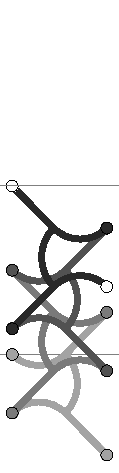
\includegraphics[scale=1]{../Pics/py/straight_f_ori_1.pdf}&
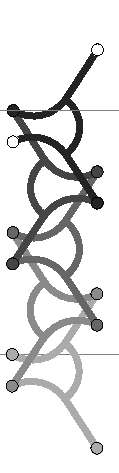
\includegraphics[scale=1]{../Pics/py/straight_f_ori_01.pdf}&
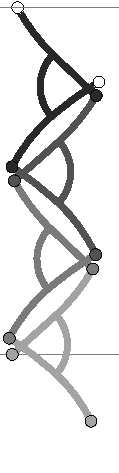
\includegraphics[scale=1]{../Pics/py/straight_f_ori_0001.pdf} \\
(a) & (b) & (c) \\
%\end{tabular}
%
%\begin{tabular}{ccc}
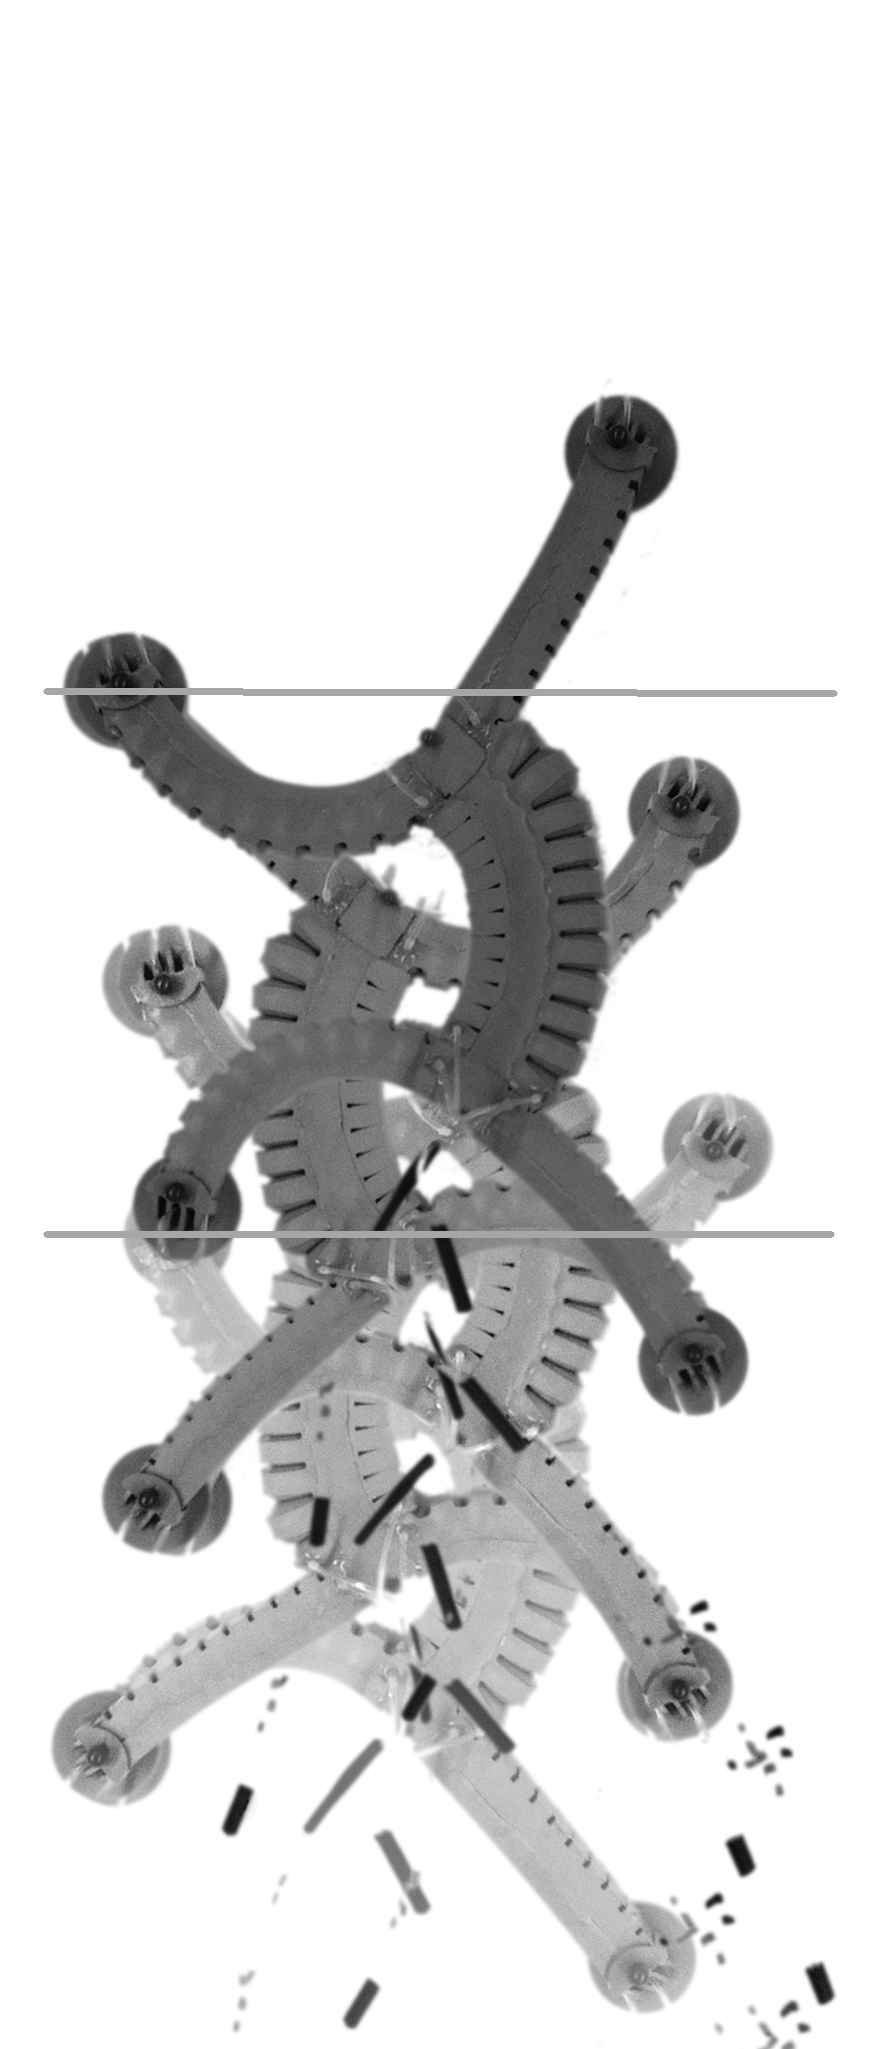
\includegraphics[width=2.45cm]{../Pics/experiment/straight_a.png}&
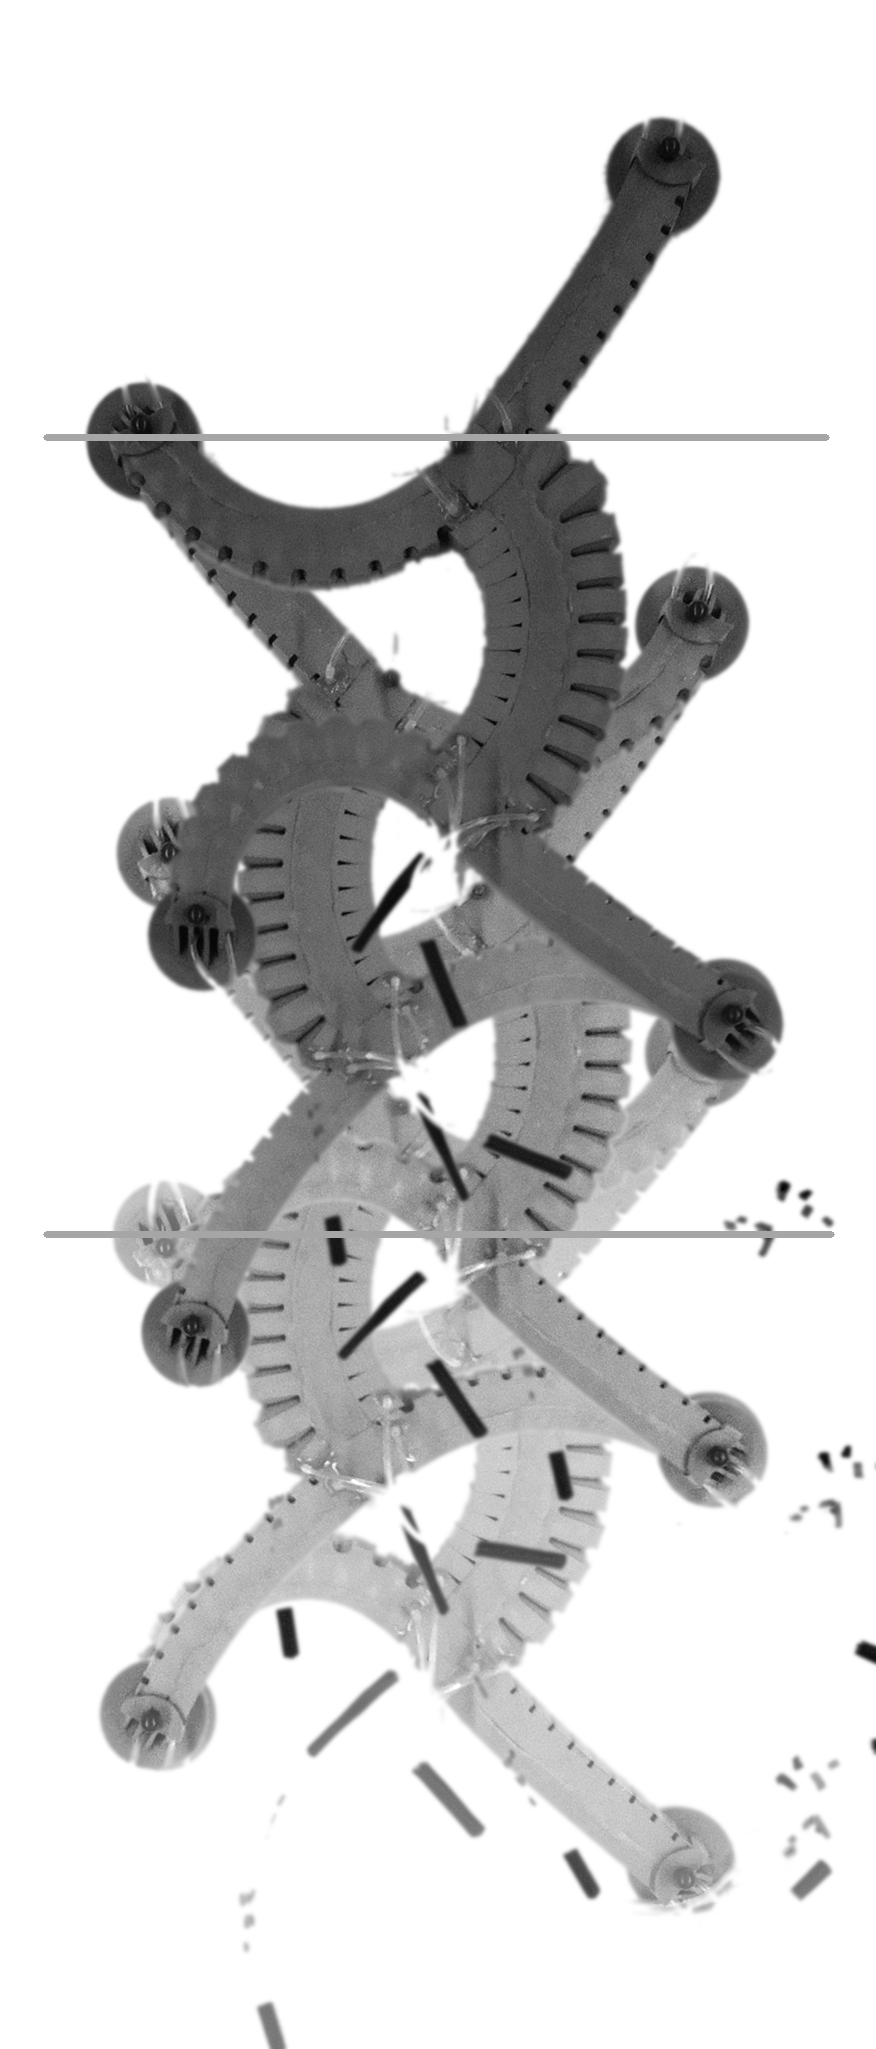
\includegraphics[width=2.45cm]{../Pics/experiment/straight_b.png}&
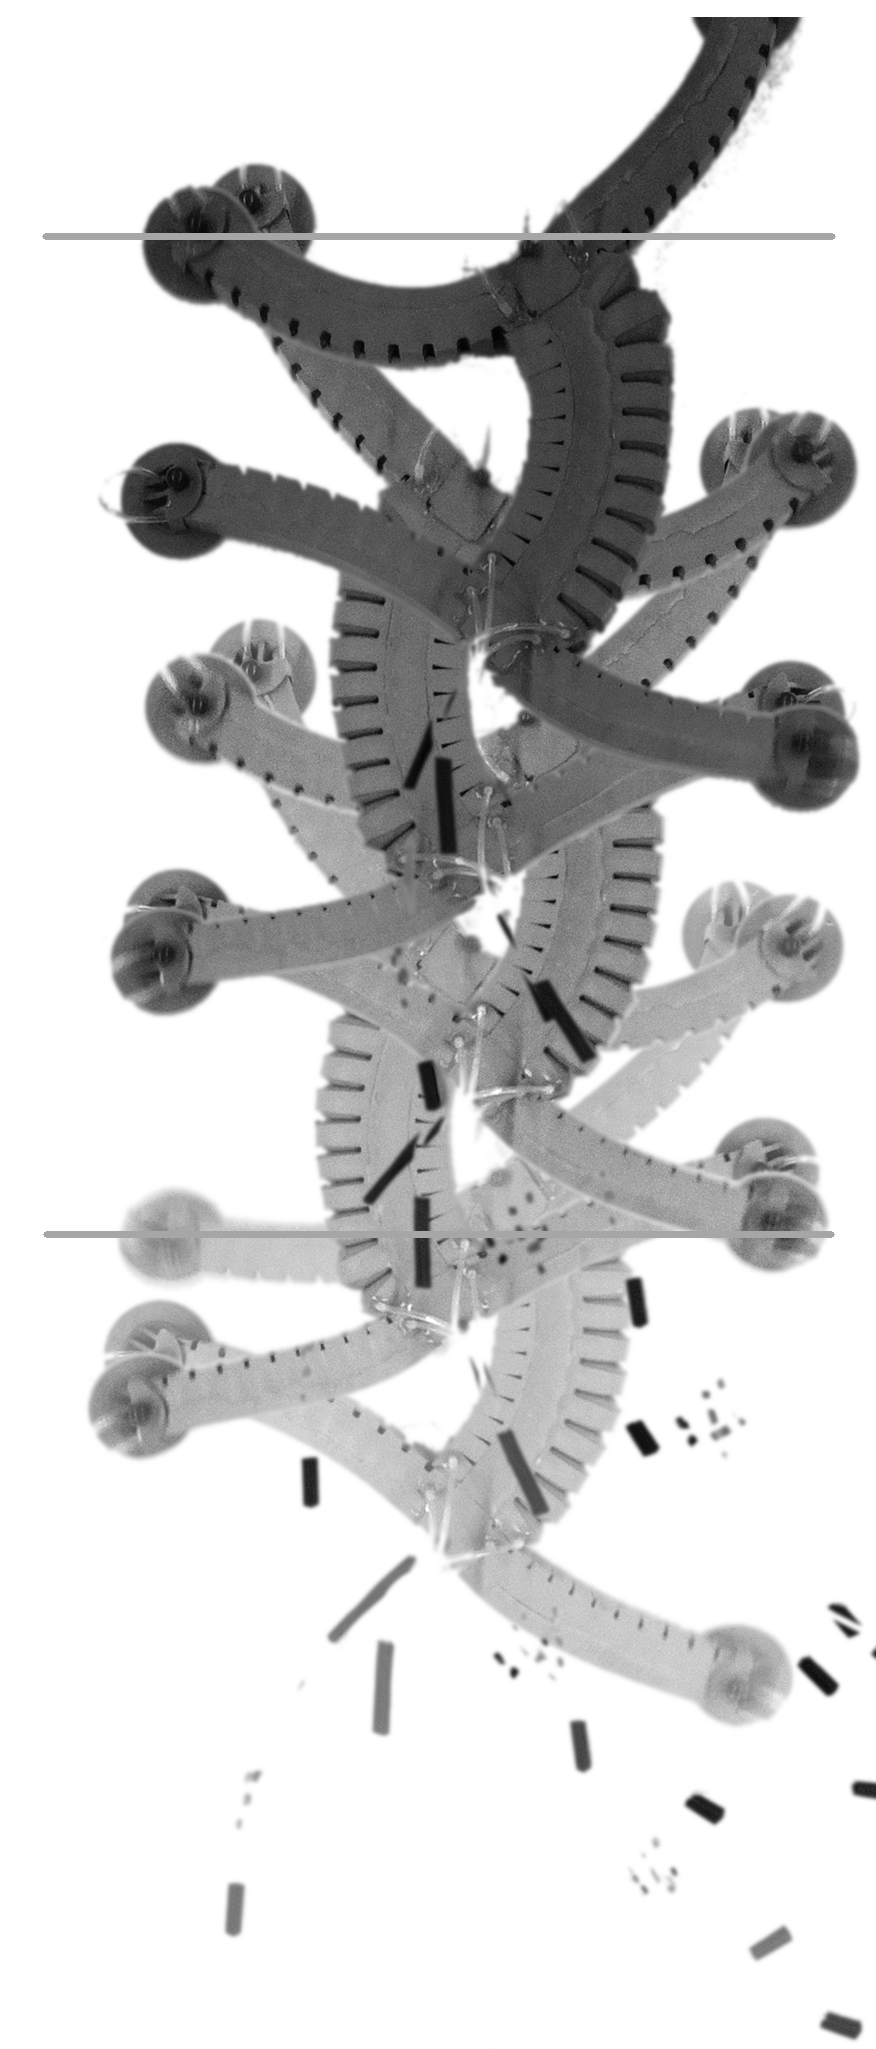
\includegraphics[width=2.45cm]{../Pics/experiment/straight_c.png} \\
(d) & (e) & (f)\\
\end{tabular}


\caption{Optimal straight gait patterns $\bm{R}_\mathcal{S}^2(\bm{y})$ for different parameter sets $\mathcal{P} = [b_\alpha, b_\ell, w_\ell, w_\alpha, w_\varphi]$.
(a) $w_\varphi = 1$, $\bm{y}=[90^\circ~0^\circ~-90^\circ~90^\circ~0^\circ]$.
(b) $w_\varphi = .1$, $\bm{y}=[86^\circ~4^\circ~-110^\circ~83^\circ~4^\circ]$.
(c) $w_\varphi = .0001$, $\bm{y}=[0^\circ~18^\circ~-85^\circ~10^\circ~22^\circ]$.
(d)--(f) the corresponding experiment for the gait pattern.}
\label{fig:opt_straight_gait}
\end{center}
\end{figure}


\subsection{Case Study: Straight Gait}

%Da bisher keine Werte für das Parameterset $\mathcal{P}$ bekannt sind, lässt sich auch keine Aussage darüber treffen, was nun wirklich das optimale Laufmuster für den geraden Gang ist.
%Deshalb wurde für jedes der drei Laufmuster jeweils ein Experiment durchgeführt.
%Da der Roboter und somit auch das Parameterset in allen Experimenten gleich bleibt, lässt sich so ermitteln, welche konkreten Werte am ehesten für das Parameterset gelten.
%Zeigt der Roboter im Experiment ein ähnliches Verhalten wie in der Simulation für ein bestimmtes Parameterset, liegt der Schluss nahe, dass dieses Parameterset die Realität wiederspiegelt.
%Wenn Simulation und Experiment weit auseinanderliegen, kann davon ausgegangen werden, dass das Parameterset falsch ist.
%
Since no values for the parameter set $\mathcal{P}$ are known so far, no statement can be made about what is really the optimal straight gait pattern.
Therefore, one experiment was performed for each of the three running patterns.
Since the robot and thus also the parameter set remain the same in all experiments, it is possible to determine which concrete values apply best to the parameter set.
If the robot shows a similar behaviour in the experiment as in the simulation for a certain parameter set, it can be concluded that this parameter set reflects reality.
If simulation and experiment are far apart, it can be assumed that the parameter set is incorrect.


%Im Experiment wurde bei jedem Wechsel der Fußfixierung automatisch ein Bild aufgenommen. 
%Diese Einzelbilder wurden übereinander gelegt und ebenfalls farbcodiert, sodass ein Vergleich mit der Simulation einfach möglich ist.
%Die Abbildungen~\ref{fig:opt_straight_gait}~(d)--(f) zeigen die Ergebnisse.
%Wieder wurde die Start- und Endposition des linken Vorderfuß durch eine horizontale Linie hervorgehoben.
%Vergleicht man (a) und (d) stellt man fest, dass der Vorschub im Experiment etwa nur halb so groß ist, wie in der Simulation.
%Das hier vorgestellte Modell berücksichtigt keinerlei Reibungseffekte oder sonstige äußere  Krafteinflüsse.
%So lässt sich dieser gewaltige Unterschied erklären.
%Die Posen des Roboters hingegen sind in Experiment und Simulation fast identisch.
%Dies spricht für die Gültigkeit dieses Parametersets.
%
In the experiment, an image was automatically taken each time the feet fixation were changed.These individual images were superimposed and also color-coded so that a comparison with the simulation is easily possible.
The figures~\ref{fig:opt_straight_gait}~(d)--(f) show the results.
Again, the start and end position of the left forefoot was marked by a horizontal line.
If we compare (a) and (d), we find that the shift in position in the experiment is only about half as high as in the simulation.
The model presented here does not consider any friction effects or other external force influences.
This is how this huge difference can be explained.
The robot's poses, on the other hand, are almost identical in experiment and simulation.
This speaks for the validity of this parameter set.


%Die Posen im Experiment mit dem optimalen Laufmuster für etwas elastische Fußgelenke in (e) zeigen eine kleine Abweichung zu denen in der Simulation (b).
%Zum einen ist der Roboter nicht in der Lage einen Verformungswinkel des Torso von $110^\circ$ zu erreichen, da das Material sonst beschädigt werden könnte.
%Zum anderen -- und das ist interessant -- ist die Abweichung der Fußorientierung zwischen den einzelnen Posen im Experiment ein wenig kleiner als in der Simulation.
%Dies bedeutet, dass der Gewichtungsfaktor $w_\varphi = .01$ ein bisschen zu niedrig ist.
%Nichts desto trotz zeigt dieses Experiment, dass die Fußorientierung durchaus einen gewissen Spielraum besitzt und durch dessen Ausnutzung ein Vorschub erzeugt werden kann, der knapp $1.5 \times$ so hoch ist, wie in (d).
%
The poses in the experiment with the optimal gait pattern for slightly elastic ankles in (e) show a small deviation from those in the simulation (b).
First, the robot is not able to achieve a torso bending angle of $110^\circ$, otherwise the material could be damaged.
On the other hand -- and this is interesting -- the deviation of the foot orientation between the individual poses in the experiment is a little smaller than in the simulation.
This means that the weighting factor $w_\varphi = 0.1$ is a bit too low.
However, it also shows that the parameter set in (a) is selected too conservatively, since the foot orientation has a certain margin and by using it, a shift in position can be generated that is around $1.5 \times$ as high as in (d).
Note that the same improvement also occurs in the simulation (b) compared to (a).

%Wie vermutet zeigt der Roboter im Experiment für frei bewegliche Fußgelenke in (f) deutlich anderes Verhalten als die Simulation in (c).
%Die einzelnen Posen sind nur mit viel Phantasie wieder zu erkennen.
%Dennoch konnte etwa $1.9 \times$ mehr Vorschub generiert werden als im Experiment in (d).
%Trotzdem ist dieses Laufmuster ungeeignet, da innerhalb der Posen große innere Spannung im Roboter herschen.
%Dies lässt sich daran erkennen, dass ein soeben losgelöstes Bein abrupt in die Ruhelage ausschlägt.
%Vergleicht man die Start- und Endpose in (f), so stellt man fest, dass sich diese wesentlich unterscheiden.
%Der Abstand zwischen den beiden linken Füßen ist in der Endpose wesentlich größer als in der Startpose.
%Auch dies ist ein Anzeichen dafür, dass dieses Laufmuster nicht wirklich stabil ist und somit nicht kontrollierbar.
%
As assumed, the robot in the experiment for freely movable ankles in (f) shows clearly different behaviour than the simulation in (c).
The individual poses can only be recognized with a lot of imagination.
Nevertheless, about $1.9 \times$ more feed could be generated than in the experiment in (d).
Nevertheless, this running pattern is unsuitable, as there is great inner stress in the robot within the poses.
This can be seen from the fact that a leg that has just been released abruptly deflects into the rest position.
If one compares the start and end poses in (f), you will notice that they differ considerably.
The distance between the two left feet is much greater in the end pose than in the starting pose.
This is also an indication for the instability of this gait pattern.


\subsection{Gait Pattern for a curve}
%Im Gegensatz zum gradlinigen Gang, ist das Laufmuster einer Kurve nicht symmetrisch.
%Die Annahme, dass ein Zyklus aus zwei Posen mit jeweils diagonal gegenüberliegend fixierten Füßen besteht, ist jedoch weiterhin sinnvoll.
%Dementsprechend hat das Laufmuster einer Kurve zehn Unbekannte, nämlich die Referenzwinkel der beiden Posen eines Zyklus.
%Die zu optimierende Variable ergibt sich damit zu:
In contrast to the straight motion, the gait pattern of a curve is not symmetrical.
However, it still reasonable to assume that a cycle consists of two poses, each with diagonally opposite fixed feet.
Accordingly, the running pattern of a curve has ten unknowns, namely the reference angles of the two poses of a cycle.
This results in the variable to be optimized:
\begin{equation}
\bm{z} = 
%\begin{bmatrix}
%\bm{z}_1 \\ \bm{z}_2
%\end{bmatrix}
%=
\begin{bmatrix}
\begin{matrix}
\alpha_{\textnormal{ref},1}& \alpha_{\textnormal{ref},2}&\alpha_{\textnormal{ref},3}&\alpha_{\textnormal{ref},4}&\alpha_{\textnormal{ref},5}
\end{matrix}
 \\
\begin{matrix}
\alpha_{\textnormal{ref},6}& \alpha_{\textnormal{ref},7}&\alpha_{\textnormal{ref},8}&\alpha_{\textnormal{ref},9}&\alpha_{\textnormal{ref},10}
\end{matrix}
\end{bmatrix} .
\end{equation}
%Wie zuvor kann nun die Struktur des Laufmuster einer Kurve mit $n$ Zyklen $\bm{R}_\mathcal{C}^n \in \mathbb{R}^{2n\times 9}$definiert werden:
As before, the structure of the gait pattern of a curve with $n$ cycles $\bm{R}_\mathcal{C}^n \in \mathbb{R}^{2n\times 9}$ can now be defined as:
\begin{equation}
\bm{R}_\mathcal{C}^n(\bm{z})
=
%\left[
%\begin{array}{c}
%\bm{r}_1 \\
%\bm{r}_2 \\
%\hline
%\bm{r}_3 \\
%\bm{r}_4 \\
%\hline
%\vdots \\
%\hline
%\bm{r}_{2n-1} \\
%\bm{r}_{2n} \\
%\end{array}
%\right]
%=
\left[
\begin{array}{ccccc cccc}
z_1&z_2&z_3&z_4&z_5&1&0&0&1 \\
z_6&z_7&z_8&z_9&z_{10}&0&1&1&0 \\ 
\hline
z_1&z_2&z_3&z_4&z_5&1&0&0&1 \\
z_6&z_7&z_8&z_9&z_{10}&0&1&1&0 \\ 
\hline
\vdots&\vdots&\vdots&\vdots&\vdots&\vdots&\vdots&\vdots&\vdots \\
\hline
z_1&z_2&z_3&z_4&z_5&1&0&0&1 \\
z_6&z_7&z_8&z_9&z_{10}&0&1&1&0 \\ 
\end{array}
\right] .
\label{eq:gait_ptrn_curve}
\end{equation}

%Um eine Kurve zu laufen ist es optimal die Differenz zwischen der Orientierung der Initialpose $\varepsilon_0$ und jener der Endpose nach $n$ Zyklen $\varepsilon_{2n}$ möglichst zu maximieren bzw. minimieren, je nach dem ob eine Links- oder Rechtskurve gelaufen werden soll.
%Zur Bestimmung der Initialpose $\bm{\rho}_0$ werden die Referenzwinkel der ersten Pose $\bm{z}_1$ des gesuchten Laufmusters $\bm{R}_\mathcal{C}(\bm{z})$ in gleicher Weise verwendet, wie dies schon beim geraden Gang geschah.
%Nun kann die Performance eines Laufmusters für eine Kurve mit $n$ Zyklen mittels folgender Funktion quantifiziert werden:
To run a curve it is optimal to maximize or minimize the difference between the orientation of the initial pose $\varepsilon_0$ and that of the end pose after $n$ cycles $\varepsilon_{2n}$, depending on whether a left or right curve is to be run.
To define the initial pose $\bm{\rho}_0$, the reference angles of the first pose $\bm{z}_1$ of the searched gait pattern $\bm{R}_\mathcal{C}(\bm{z})$ are used in the same way as it already happened for straight gait.
Now the performance of a gait pattern for a curve with $n$ cycles can be quantified using the following objective:
\begin{equation}
\Delta\varepsilon^n(\bm{z})
 = 
\left\lbrace
\begin{array}{l}
\bm{\rho}_0 = 
\left[
\begin{array}{c|c|c}
\bm{z}_1 ~ \bm{\ell}_n ~ \varepsilon_0  & 
\bm{P}(\bm{z}_1, \bm{\ell}_n, \varepsilon_0, \bm{p}_{1,0}) & 
1~0~0~0
\end{array}
\right] \\
\textnormal{for } k = 1, \dots, 2n: \\
\qquad \bm{\rho}_k = \textnormal{fun}_{\mathcal{P}}(\bm{r}_k, \bm{\rho}_{k-1}) \\
\Delta \varepsilon = \varepsilon_{2n} - \varepsilon_0 \\
\end{array}
\right. .
\end{equation}

%Das Optimale Laufmuster für eine Linkskurve zu einem gegebenen Parameterset $\mathcal{P}$ ist dann die Lösung des Optimierungsproblems:
The optimal gait pattern for a left curve to a given parameter set $\mathcal{P}$ is then the solution to the optimization problem:
\begin{equation}
\min_{\bm{z} \in \mathcal{Z}} ~ -\Delta\varepsilon^n(\bm{z}).
\end{equation}
Here $\mathcal{Z}$ describes the set of allowed values.
All reference angles of the legs should be $z_i\geq0,~i=1,2,4,5,6,7,9,10$. 
The reference angles of the torso $z_i,~i=3,8$ are not constrained, since it can bend into both directions.
%Für eine Rechtskurve multipliziert man die Kostenfunktion mit $-1$.
For a right turn, multiply the objective function by $-1$.
%Zur Lösung des Minimierungsproblems wird wieder ein Startwert benötigt.
%Dafür wird $\bm{z}_0 = [\bm{y}_0~\bm{y}_0]$ gewählt.
A starting value is required again to solve the minimization problem.
Therefore $\bm{z}_0 = [\bm{y}_0~\bm{y}_0]$ is chosen.


%Abbildung~\ref{fig:opt_curve_gait} zeigt die Ergebnisse der Optimierung für verschiedene Parametersets $\mathcal{P}$.
%Es sind jeweils die vier Posen von zwei Zyklen und die erste Pose des dritten Zyklus dargestellt.
%Die Grenzen, sowie die Kosten für Winkel- und Längenabweichung sind in allen Simulationen konstant $[b_\alpha, b_\ell, w_\ell, w_\alpha] = [100^\circ, .1, 100, 10]$.
%Wieder wurden nur die Kosten für die Orientierungsabweichung der fixierten Füße $w_\varphi$ variiert.
%Die ersten drei Abbildungen (a)--(c) zeigen optimale Linkskurven ($\min -\Delta \varepsilon$).
%In ist ein Verdrehen der Füße relativ teuer $w_\varphi=1$.
%Innerhalb der 2.5 Zyklen konnte eine Rotation von $45^\circ$ generiert werden, was $18^\circ/$cycle entspricht.
%Man beachte, dass die Orientierung der fixierten Füße nahezu konstant bleibt.
%In (b) wurden die Kosten für das Verdrehen der Füße etwas gesenkt ($w_\varphi=.1$).
%Die Orientierungsabweichung der fixierten Füße ist nun zwar etwas größer, dafür wurde aber eine Rotation von $30^\circ/$cycle erzeugt, und damit fast Doppelt soviel wie in (a).
%In (c) besitzt der Roboter quasi voll bewegliche Fußgelenke ($w_\varphi=.0001$).
%In den den 2.5 Zyklen rotiert er um $235^\circ \hat{=} 94^\circ/$cycle.
%Allerdings beinhaltet dieses Laufmuster Biegewinkel von bis zu $221^\circ$, sodass es praktisch schwer umzusetzen ist.

Figure~\ref{fig:opt_curve_gait} shows the optimization results for different parameter sets $\mathcal{P}$.
The four poses of two cycles and the first pose of the third cycle are shown.
The limits and costs for angle and length deviation are constant $[b_\alpha, b_\ell, w_\ell, w_alpha] =[100^\circ, .1, 100, 10]$ in all simulations.
Again, only the cost of the orientation deviation of the fixed feet $w_\varphi$ was varied.
The first three figures (a)--(c) show optimal left curves ($\min -\Delta \varepsilon$).
In (a), twisting of the feet is relatively expensive $w_\varphi=1$.
Within the 2.5 cycles a rotation of $45^\circ$ could be generated, which corresponds to $18^\circ/$cycle.
Note that the orientation of the fixed feet remains almost constant.
In (b) the cost of twisting the feet was slightly reduced ($w_\varphi=.1$).
The orientation deviation of the fixed feet is now slightly larger, but a rotation of $30^\circ/$cycle was generated, almost twice as much as in (a).
In (c) the robot has fully movable ankle joints ($w_\varphi=.0001$).
In the 2.5 cycles it rotates around $235^\circ \hat{=} 94^\circ/$cycle.
However, this gait pattern has bending angles of up to $221^\circ$, making it practically difficult to move.

To convert a gait pattern for a left curve into that for a right curve, the reference angles must be mirrored.
The mirror image $\tilde{\bm{r}}$ of a reference input $\bm{r}$ is defined as:
\begin{equation}
\tilde{\bm{r}}(\bm{r}) = \begin{bmatrix}
r_2 & r_1 & - r_3 & r_5 & r_4  & \bm{f}^\top
\end{bmatrix} .
\end{equation}
If the mirroring is applied to all poses of the gait pattern for left turns, the robot runs forward right.


\begin{figure}
\begin{center}
\begin{tabular}{cc}
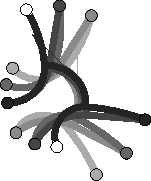
\includegraphics[scale=1]{../Pics/py/Curve_f_ori_1.pdf}&
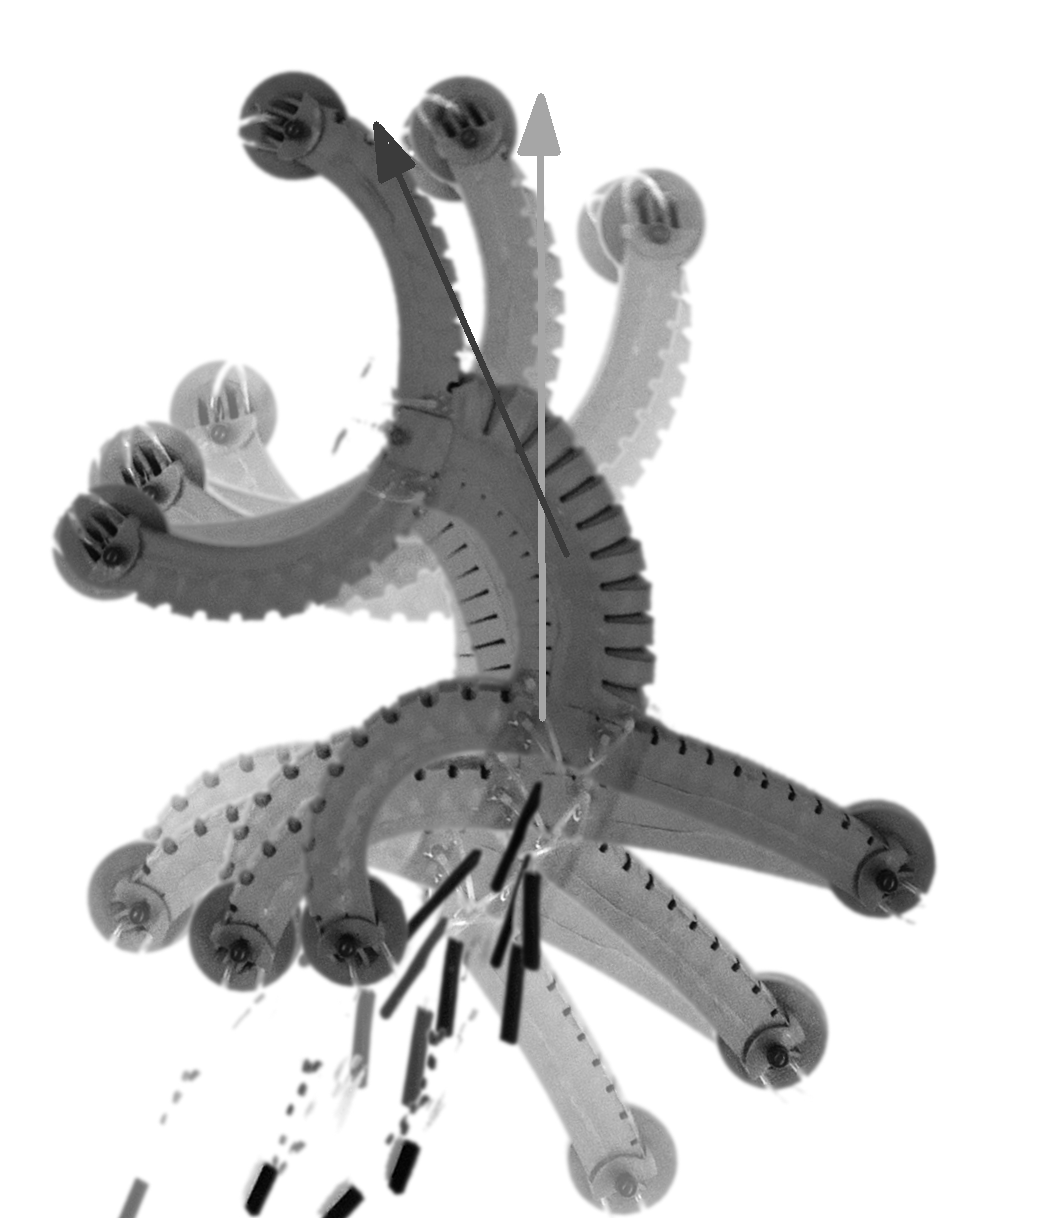
\includegraphics[width=3cm]{../Pics/experiment/curve_a.png} \\
(a) & (d) \\ 
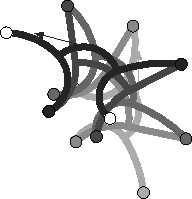
\includegraphics[scale=1]{../Pics/py/Curve_f_ori_01.pdf}&
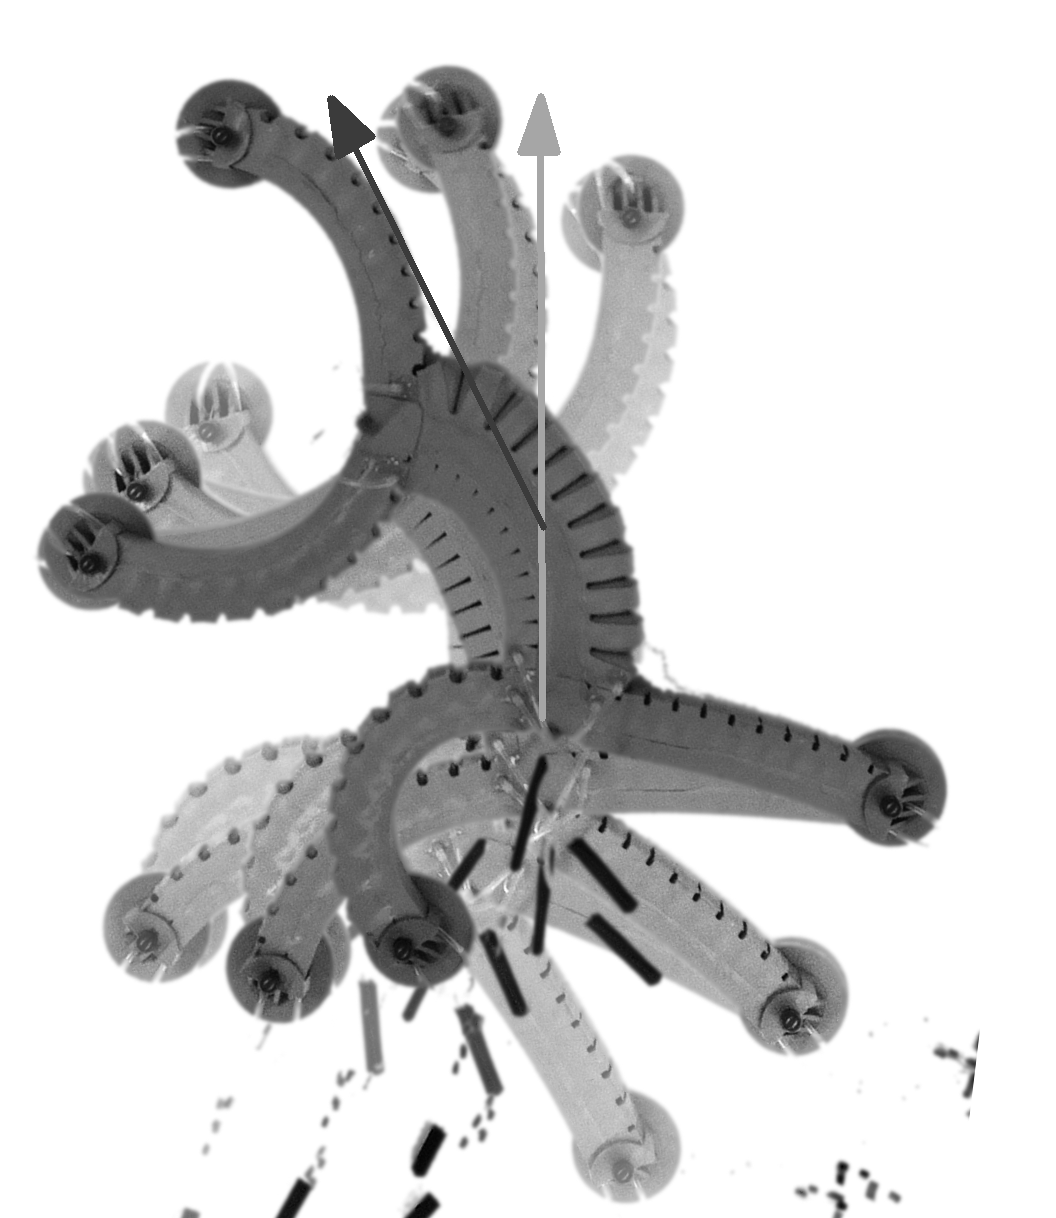
\includegraphics[width=3cm]{../Pics/experiment/curve_b.png} \\
(b) & (e) \\
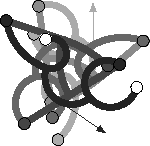
\includegraphics[scale=1]{../Pics/py/Curve_f_ori_0001.pdf} &
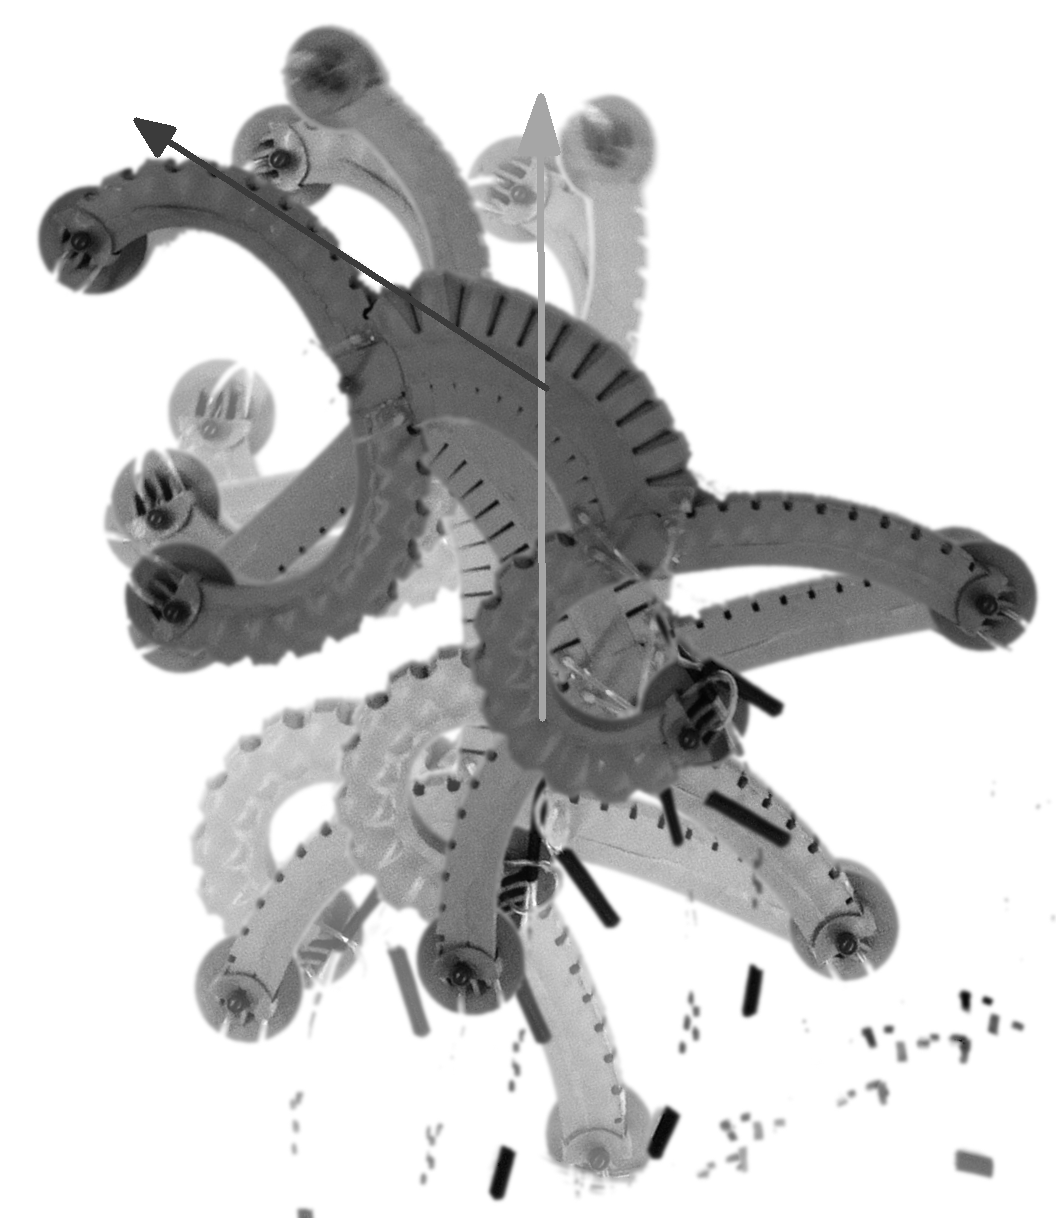
\includegraphics[width=3cm]{../Pics/experiment/curve_c.png} \\
(c) & (f) \\
\end{tabular}

%\begin{tabular}{ccc}
%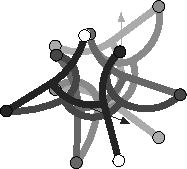
\includegraphics[scale=1]{../Pics/py/U-turn_f_ori_1.pdf}&
%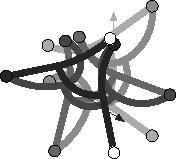
\includegraphics[scale=1]{../Pics/py/U-turn_f_ori_01.pdf}&
%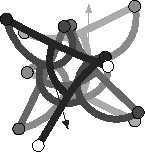
\includegraphics[scale=1]{../Pics/py/U-turn_f_ori_0001.pdf} \\
%(d) & (e) & (f)\\
%\end{tabular}

\caption{
Optimal left curve gait patterns $\bm{R}_\mathcal{C}^2(\bm{z})$ for different parameter sets $\mathcal{P} = [b_\alpha, b_\ell, w_\ell, w_\alpha, w_\varphi]$ ($\min -\Delta\varepsilon$):
(a) $w_\varphi = 1$, $\bm{z}=[[97^\circ~28^\circ~-98^\circ~116^\circ~17^\circ]~[79^\circ~0^\circ~-84^\circ~67^\circ~0^\circ]$.
(b) $w_\varphi = .1$, $\bm{z}=[[104^\circ~48^\circ~-114^\circ~124^\circ~27^\circ]~[72^\circ~0^\circ~-70^\circ~55^\circ~0^\circ]$.
(c) $w_\varphi = .0001$, $\bm{z}=[[164^\circ~124^\circ~-152^\circ~221^\circ~62^\circ]~[0^\circ~0^\circ~-24^\circ~0^\circ~0^\circ]$.
%Optimal right curve gait patterns ($\min \Delta\varepsilon$):
%(d) $w_\varphi = 1$, $\bm{z}=[[63^\circ~0^\circ~-72^\circ~46^\circ~0^\circ]~[114^\circ~77^\circ~-121^\circ~144^\circ~31^\circ]$.
%(e) $w_\varphi = .01$, $\bm{z}=[[60^\circ~0^\circ~-70^\circ~30^\circ~0^\circ]~[110^\circ~70^\circ~-132^\circ~149^\circ~43^\circ]$.
%(f) $w_\varphi = .001$,  $\bm{z}=[[50^\circ~0^\circ~-51^\circ~6^\circ~0^\circ]~[121^\circ~92^\circ~-146^\circ~167^\circ~54^\circ]$.
(d)--(f) the corresponding experiment for the gait pattern.
}
\label{fig:opt_curve_gait}
\end{center}
\end{figure}



\subsection{Case Study: Gait Pattern for a curve}

%Wie zuvor werden auch die verschiedenen Laufmuster für eine Kurve im Experiment getestet.
%Das Experiment ist gleich aufgebaut wie das für den geraden Gang.
%Die Abbildungen~\ref{fig:opt_curve_gait}~(d)--(f) zeigen das Resultat.
%Vergleicht man das Experiment in (d) mit der Simulation in (a) lässt sich der wesentliche Unterschied feststellen, dass im Experiment innerhalb der 2.5 Zyklen etwa nur halb soviel Rotation erzeugt wurde wie in der Simulation ($25^\circ$ statt $45^\circ$).
%Dieser Faktor von 2 ist uns schon aus dem Vergleich von Simulation und Experiment des geraden Ganges bekannt.
%Auch hier sei auf die fehlende Modellierung von Reibung hingewiesen.
%Die Posen hingegen entsprechen weitestgehend der Simulation.
%Auch die Abweichung der Fußorientierung zwischen den einzelnen Posen ist sehr gering, wie vom Parameterset gefordert ($w_\varphi=1$).
%
As before, the different gait patterns for a curve are also tested in the experiment.
The experiment is structured in the same way as for the straight gait.
The figures~\ref{fig:opt_curve_gait}~(d)--(f) show the result.
Comparing the experiment in (d) with the simulation in (a), the main difference is that the robot in the  experiment generated about half as much rotation within the 2.5 cycles as in the simulation ($25^\circ$ instead of $45^\circ$).
We already know this factor of 2 from the comparison of simulation and experiment of the straight gait.
Again, the lack of modelling of friction should be pointed out.
The poses, on the other hand, are almost identical to the simulation.
The deviation of the foot orientation between the individual poses is also very small, as demanded by the parameter set ($w_\varphi=1$).
%
%Im zweiten Experiment (e) wird nicht wesentlich mehr Rotation erzeugt wie im ersten ($28^\cric$).
%Verglichen mit der Simulation ist das etwa nur ein Drittel.
%Die Abweichung der Fußorientierung ist wesentlich niedriger als in der Simulation, jedoch ein wenig höher als im ersten Experiment (a).
%Dies lässt wiederum den Schluss zu, dass das Parameterset aus (a) zu konservativ ist und das aus (b) zu locker gewählt.
%

In the second experiment (e) not much more rotation is generated ($28^\circ$) than in the first.
Compared to the simulation (b), this is only about a third.
The deviation of the foot orientation is considerably lower than in the simulation, but slightly higher than in the first experiment (a).
This in turn leads to the conclusion that the parameter set from (a) is too conservative and that from (b) is too loose.
%
%Im dritten Experiment wurde gut doppelt soviel Rotation erzeugt wie in den beiden ersten ($55^\circ$).
%Die Posen stimmen weitestgehend mit der SImulation überein.
%Allerdings ist zu beachten, dass sie die Position der fixierten Füße verändern.
%Dies lässt sich nur dadurch erklären, dass die Füße nicht über den gesamten Bewegungszeitraum fixiert waren.
%Besonders gut zu erkennen ist das am vorderen rechten und am hinteren linken Fuß.
%Durch die starke Aktuierung der Beine verformt sich der Saugnapf an dessen Ende und eine Fixierung ist nicht mehr sichergestellt.
%Wird das Experiment auf einer horizontalen Ebene durchgeführt, hat dies keinen großen Einfluss.
%Auf einer vertikalen Wand hingegen, entscheidet das über den Absturz.
%

In the third experiment twice as much rotation was generated as in the first two ($55^\circ$).
The poses match the simulation.
However, it should be noted that the fixed feet change position.
This can only be explained by the fact that the feet were not fixed over the entire movement period.
This can be seen particularly well on the front right and rear left foot.
Due to the strong actuation of the legs, the suction cup deforms end and fixation is no longer ensured.
If the experiment is carried out on a horizontal plane, this has no great influence.
On a vertical wall, on the other hand, this is the deciding factor for the crash.


\section{Conclusion}

%Dieses Paper präsentiert einen Algorithmus, um die Pose des Gecko-inspirierten weichen Roboters aus \cite{PA_SCHILLER} zu einem gegebenen Referenzinput vorher zu sagen.
%Dieser Algorithmus basiert auf einem geometrischen Optimierungsproblem.
%Im Wesentlichen werden Kreisbögen derart angeordnet, dass ihre Endpunkte den Positionen der fixierten Füße entsprechen.
%Um dies erfüllen zu können, erlaubt der Algorithmus Abweichungen in der Länge der Kreisbögen, in deren Orientierung und in deren Biegewinkel.
%Die Kosten für die Abweichung werden mit Faktoren gewichtet, die auch physikalisch interpretiert werden können.
%So ist der Funktionswert der Kostenfunktion ein Maß für die innere Spannung einer Pose.
%Die Gewichtungsfaktoren werden in einem Parameterset $\mathcal{P}$ zusammengefasst.
%
%Dieser Algorithmus kann nun benutzt werden, um neue Laufmuster für den Roboter zu finden.
%Dabei wird die Struktur des Laufmusters vorgegeben.
%Für einen geraden Gang besteht die Struktur nur aus zwei spiegelsymmetrischen Posen, die in Dauerschleife wiederholt werden.
%Das optimale Laufmuster kann nun durch die Formulierung eines weiteren Optimierungsproblems gefunden werden.
%Die zu maximierende Größe ist hierbei der in einem Laufmuster mit $n$ Zyklen generierte Vorschub, welcher sich durch die rekursive Anwendung des Algorithmus berechnet lässt.
%So konnte ein stabiles Laufmuster für den geraden Gang gefunden werden, dass $1.5 \times$ mehr Vorschub generiert als das bisher bekannte.
%
%In gleicher Weise wurde der Algorithmus benutzt, um ein Laufmuster für eine Kurve zu finden.
%Dabei war die zu maximierende Größe die Orientierung des Torso.
%Auch hier konnte ein stabiles Laufmuster entdeckt werden, dass den Roboter dazu befähigt, sich auf der Stelle zu drehen.
%
%Mit diesem Wissen lassen sich nun beliebige Trajekorien ablaufen, da jede Kurve als Kombination aus Geraden und Kreisbögen mit unterschiedlichen Radien beschrieben werden kann.
%In zukünftigen Forschungsarbeiten wird der Fokus auf Spurverfolgung liegen.




This paper presents an algorithm to predict the pose of the gecko-inspired soft robot from \cite{PA_SCHILLER} for a given reference input.
This algorithm is based on a geometric optimization problem.
Essentially, arcs are arranged so that their end points correspond to the positions of the fixed feet.
To be able to do this, the algorithm allows deviations in the length of the arcs, in their orientation and in their bending angle.
The costs for these deviations are weighted with factors that can also be interpreted physically.
Thus, the functional value of the objective function is a measure of the inner stress of a pose.
The weighting factors are summarized in a parameter set $\mathcal{P}$.

This algorithm can now be used to find new gait patterns for the robot.
In this case, the structure of the gait pattern is specified.
For a straight gait, the structure consists of only two mirror-symmetrical poses that are repeated in a continuous loop.
The optimal gait pattern can now be found by formulating a further optimization problem.
The quantity to be maximized is the shift in position generated in a gait pattern with $n$ cycles, which can be calculated by the recursive application of the algorithm.
A stable pattern for the straight gait was found that generates $1.5 \times$ more shift in position than the previously known one.

In the same way, the algorithm was used to find a gait pattern for a curve.
The quantity to be maximized was the orientation of the torso.
Again, a stable gait pattern was discovered that enables the robot to rotate on the spot.

With this knowledge, any trajectories can now be executed, since each curve can be described as a combination of straight lines and arcs with different radii.
In future research work, the focus will be on tracking arbitrary trajectories.


%%%%%%%%%%%%%%%%%%%%%%%%%%%%%%%%%%%%%%%%%%%%%%%%%%%%%%%%%%%%%%%%%%%%%%%%%%%%%%%%

\section*{APPENDIX}

\begin{equation}
r_i = \frac{360 ~ \ell_i}{2 \pi ~ \alpha_i},~~ \textnormal{for}~ i \in [1,2,3,4,5]
\label{eq:F1_start}
\end{equation}

\begin{equation}
\bm{\varphi} = \begin{bmatrix}
\varepsilon - \alpha_1 - \frac{1}{2}\alpha_3 \\
\varphi_1 + \alpha_1 + \alpha_2 \\
180^\circ + \alpha_3 - \alpha_2 + \alpha_4 + \varphi_2 \\
180^\circ + \alpha_3 - \alpha_1 + \alpha_5 + \varphi_1 \\
\end{bmatrix}
\label{eq:phi_calc}
\end{equation}

If $f_1$:

\begin{equation}
\bm{p}_{R1} = \bm{p}_1 + 
\begin{bmatrix} 
\cos(\varphi_1)\\ 
\sin(\varphi_1)\end{bmatrix} r_1
\end{equation}

\begin{equation}
\bm{p}_{OM} = \bm{p}_{R1} + \begin{bmatrix} 
\cos(\varphi_1 + \alpha_1) \\ 
\sin(\varphi_1 + \alpha_1)
\end{bmatrix} r_1
\end{equation}

\begin{equation}
\bm{p}_{R2} = \bm{p}_{OM} + 
\begin{bmatrix} 
\cos(\varphi_1 + \alpha_1) \\ 
\sin(\varphi_1 + \alpha_1)
\end{bmatrix} r_2
\end{equation}

\begin{equation}
\bm{p}_{2} = \bm{p}_{R2} + 
\begin{bmatrix} 
-\cos(\varphi_2) \\ 
-\sin(\varphi_2)
\end{bmatrix} r_2
\end{equation}



If $f_2$:

\begin{equation}
\bm{p}_{R2} = \bm{p}_{2} + 
\begin{bmatrix} 
\cos(\varphi_2) \\ 
\sin(\varphi_2)
\end{bmatrix} r_2
\end{equation}

\begin{equation}
\bm{p}_{OM} = \bm{p}_{R2} + 
\begin{bmatrix} 
-\cos(\varphi_2-\alpha_2) \\ 
-\sin(\varphi_2-\alpha_2)
\end{bmatrix} r_2
\end{equation}

\begin{equation}
\bm{p}_{R1} = \bm{p}_{OM} + 
\begin{bmatrix} 
\cos(\varphi_2-\alpha_2) \\ 
\sin(\varphi_2-\alpha_2)
\end{bmatrix} r_1
\end{equation}

\begin{equation}
\bm{p}_{1} = \bm{p}_{R1} + 
\begin{bmatrix} 
-\cos(\varphi_1) \\ 
-\sin(\varphi_1)
\end{bmatrix} r_1
\end{equation}


Both:

\begin{equation}
\bm{p}_{RM} = \bm{p}_{OM} + \begin{bmatrix} 
\sin(\varphi_1 + \alpha_1) \\ 
-\cos(\varphi_1 + \alpha_1) \end{bmatrix} r_3
\end{equation}


\begin{equation}
\bm{p}_{UM} = \bm{p}_{RM} + \begin{bmatrix} 
- \cos(\alpha_3 - 90 + \varphi_1 + \alpha_1) \\ 
- \sin(\alpha_3 - 90 + \varphi_1 + \alpha_1) \end{bmatrix} r_3
\end{equation}

\begin{equation}
\bm{p}_{R4} = \bm{p}_{UM} + \begin{bmatrix} 
\sin(\alpha_3 - 90 + \varphi_1 + \alpha_1) \\
- \cos(\alpha_3 - 90 + \varphi_1 + \alpha_1) \end{bmatrix} r_4
\end{equation}

\begin{equation}
\bm{p}_{4} = \bm{p}_{R4} + \begin{bmatrix} 
-\cos(\varphi_4) \\
-\sin(\varphi_4)\end{bmatrix} r_4
\end{equation}

\begin{equation}
\bm{p}_{R3} = \bm{p}_{UM} + \begin{bmatrix} 
\sin(\alpha_3 - 90 + \varphi_1 + \alpha_1) \\
 - \cos(\alpha_3 - 90 + \varphi_1 + \alpha_1) \end{bmatrix} r_3
\end{equation}

\begin{equation}
\bm{p}_{3} = \bm{p}_{R3} + \begin{bmatrix} 
- \cos(\varphi_3)\\
- \sin(\varphi_3)\end{bmatrix}r_3
\label{eq:F1_end}
\end{equation}











%\begin{figure}
%\begin{center}
%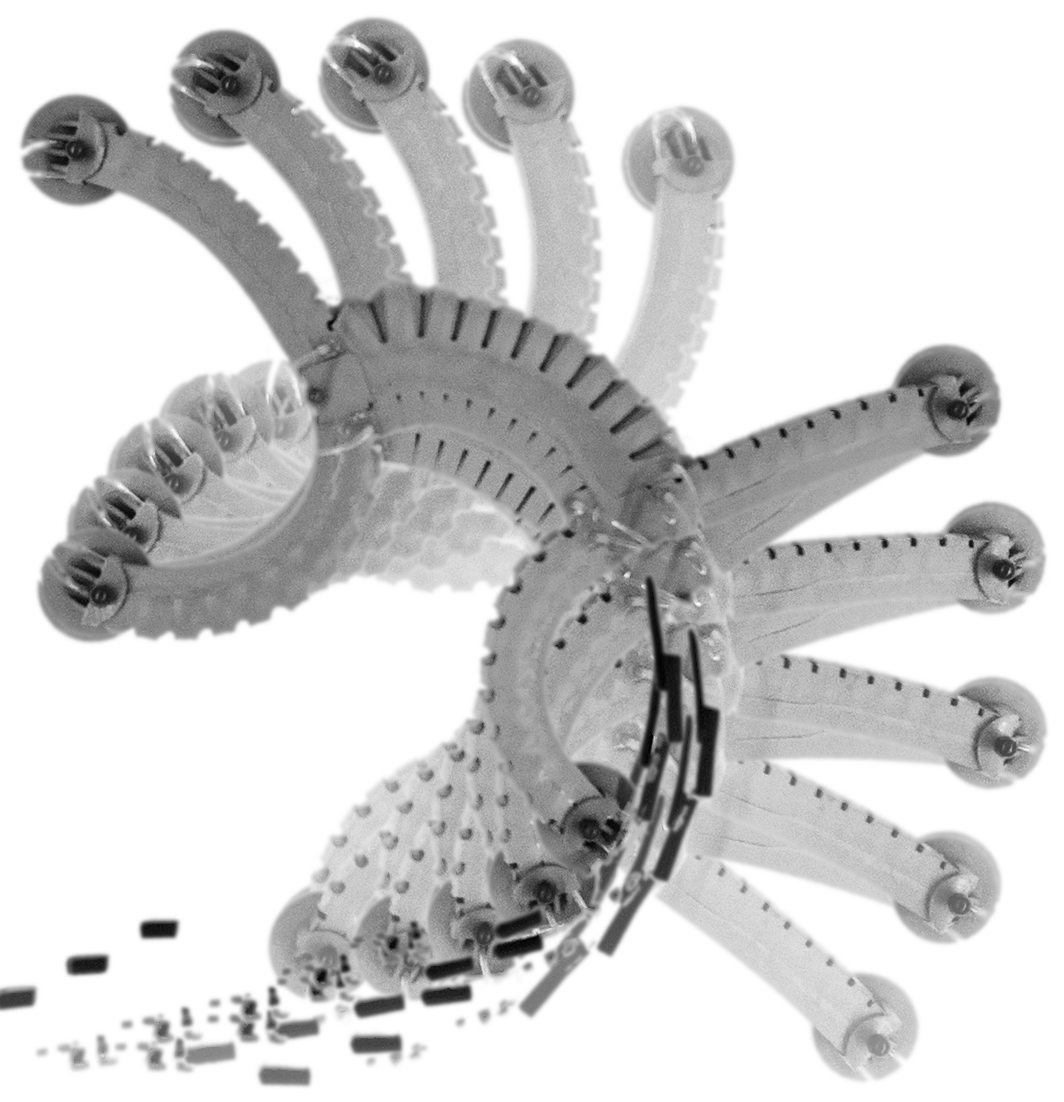
\includegraphics[width=.4\textwidth]{../Pics/experiment/curve.png}
%\caption{4 cycles of the curve pattern}
%\end{center}
%\end{figure}



%\begin{figure}
%\begin{center}
%\begin{tabular}{cc}
%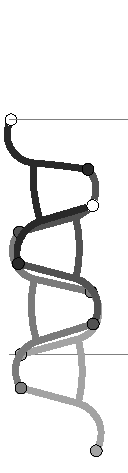
\includegraphics[scale=1]{../Pics/py/n_belly_100_10_001.pdf}&
%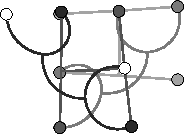
\includegraphics[scale=1]{../Pics/py/U-turn.pdf} \\
%
%(a) & (b) \\
%\end{tabular}
%
%\caption{
%(a) Optimal straight gait patterns without moving torso $\mathcal{P} = [100, .1, 100, 10, .001]$.
%(b) Optimal curve for a fixed initialpose with $\bm{\alpha}_0 = [0~0~0~0~0]$, $w_\varphi = .0001$, $\bm{z}=[[0^\circ~0^\circ~-7^\circ~0^\circ~0^\circ]~[114^\circ~109^\circ~-101^\circ~146^\circ~82^\circ]$.
%}
%\label{fig:straight_gait_no_torso}
%\end{center}
%\end{figure}



%Appendixes should appear before the acknowledgment.
%\section*{ACKNOWLEDGMENT}
%


%\addtolength{\textheight}{-.2cm}   % This command serves to balance the column lengths

%%%%%%%%%%%%%%%%%%%%%%%%%%%%%%%%%%%%%%%%%%%%%%%%%%%%%%%%%%%%%%%%%%%%%%%%%%%%%%%%
%References are important to the reader; therefore, each citation must be complete and correct. If at all possible, references should be commonly available publications.

\bibliographystyle{unsrt}
\bibliography{bib}


\end{document}